\documentclass[12pt]{standalone}

\usepackage[T1]{fontenc}
\usepackage[svgnames]{xcolor}
\usepackage{tikz}
\colorlet{Random0}{Yellow!50!DarkKhaki}
\colorlet{Random1}{Yellow!50!DarkKhaki}
\usepackage{kpfonts}
\usetikzlibrary{fadings}
\usepackage[ttdefault=true]{AnonymousPro}
%\usepackage{courier}
\usepackage{contour}
\contourlength{0.1pt} %how thick each copy is
\begin{document}
	
	
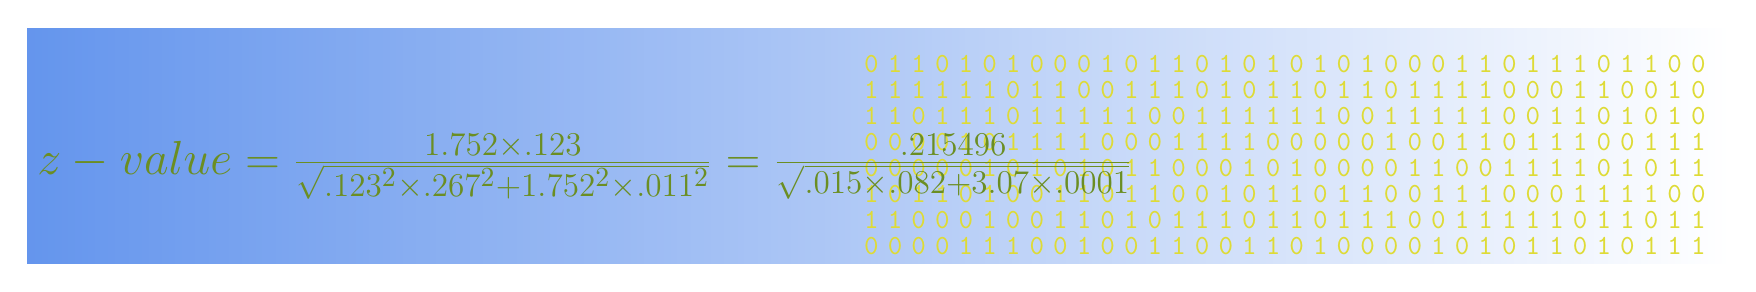
\begin{tikzpicture}[yshift=-3cm]
\path[fill=%DodgerBlue,
CornflowerBlue,
%DeepSkyBlue!70!MidnightBlue,
path fading=east] (0,0) rectangle(\paperwidth,3cm);
\foreach \x in {35,...,70}{
	\foreach \y in {0,...,7} 
	\pgfmathsetmacro\Random{random(0,1)}
	\node[draw=none,color=Random\Random,anchor=south west,font=\ttfamily\bfseries] 
	at (\x*.3cm,\y*.33cm) 
	{\Random};};
\node[anchor=south west,font=\LARGE\bfseries,yshift=0.7cm]{%\contour{Black}
	{\textcolor{OliveDrab}{$
\text{z-value}=\frac{1.752\times .123}{\sqrt{.123^2\times .267^2+1.752^2\times .011^2}}=\frac{.215496}{\sqrt{.015\times .082+3.07\times .0001}}
$}}};
\end{tikzpicture}

\end{document}
